\begin{sidewaysfigure}[htbp]
\centering 
  \subfloat[Low friction, average velocity.]
  {
	  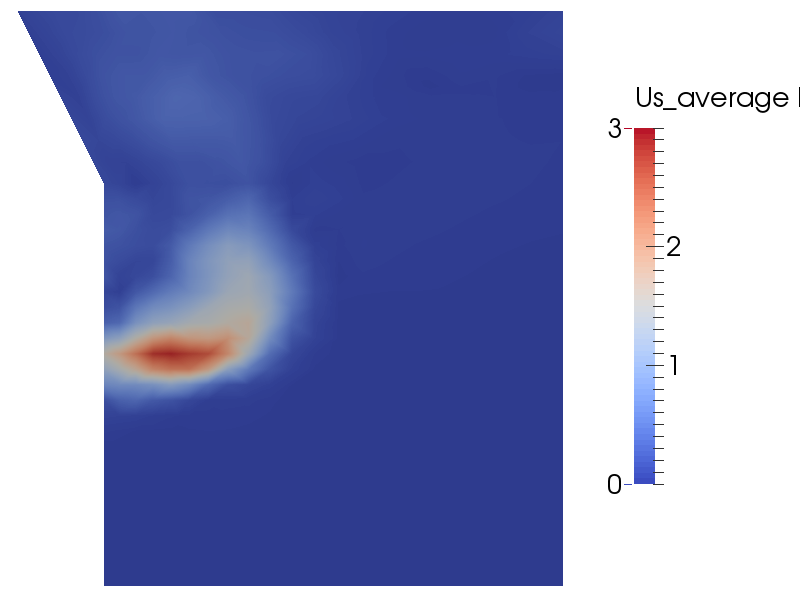
\includegraphics[width=.4\columnwidth]{images/231us_average_lf}
	  \label{fig:231us_average_lf}
  }
  \quad
    \subfloat[High friction, average velocity.]
    {
	  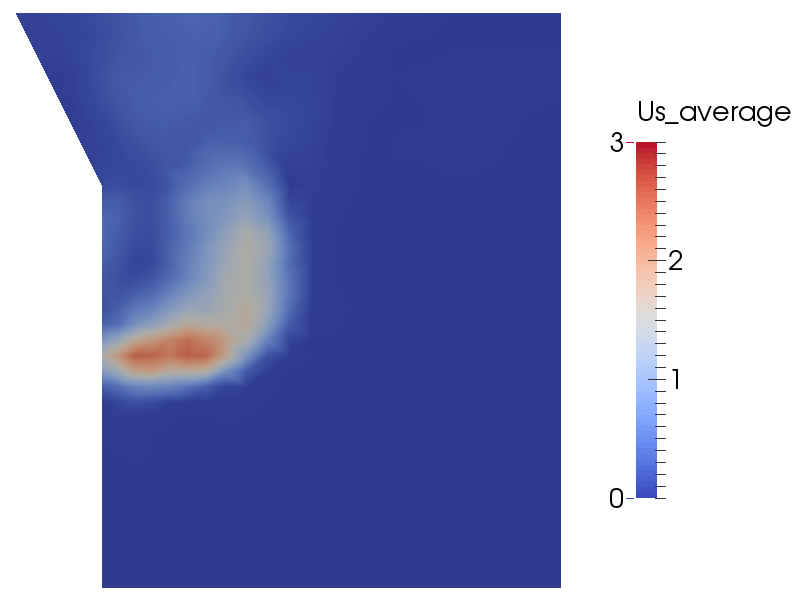
\includegraphics[width=.4\columnwidth]{images/230us_average_hf}
	  \label{fig:230us_average_hf}
  }
  \\
  \subfloat[Low friction, standard deviation velocity.]
  {
	  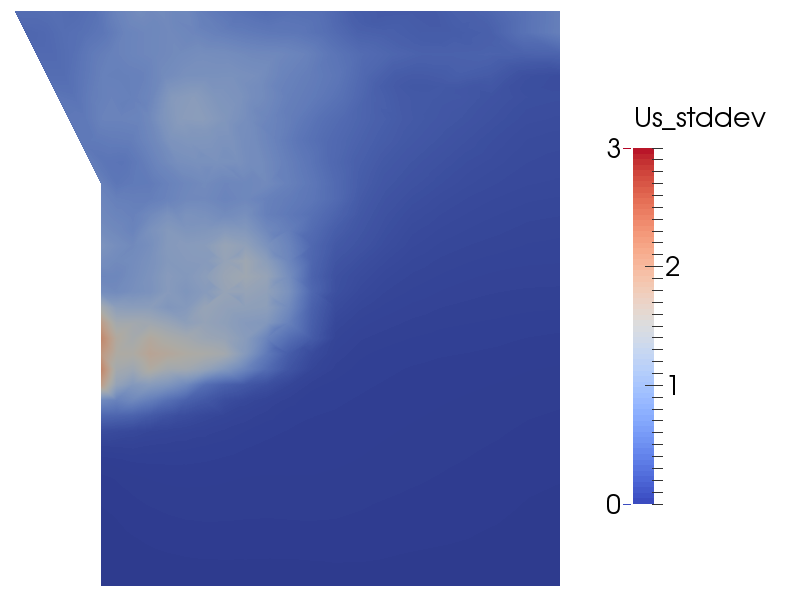
\includegraphics[width=.4\columnwidth]{images/233us_std_lf}
	  \label{fig:233us_std_lf}
  }
  \quad
    \subfloat[High friction, standard deviation velocity.]
    {
	  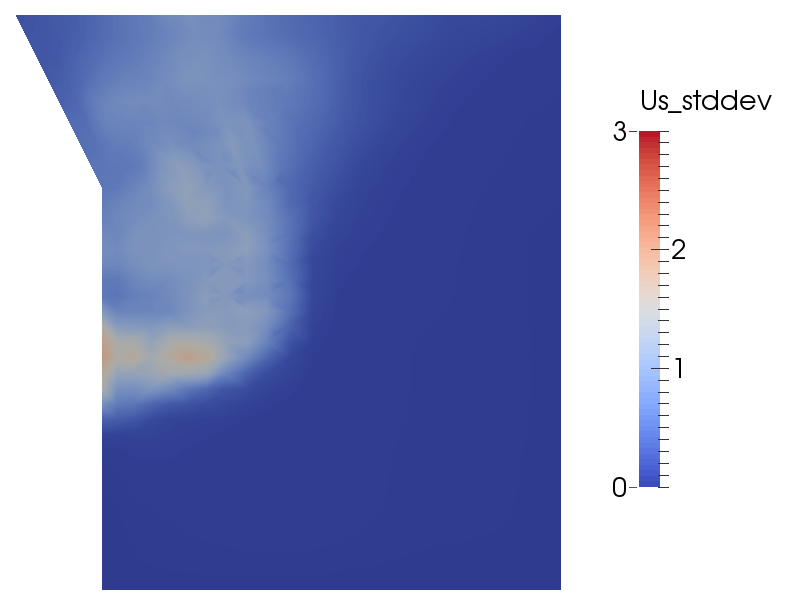
\includegraphics[width=.4\columnwidth]{images/232us_std_hf}
	  \label{fig:232us_std_hf}  }
  \\
  \caption{Particle velocity with different sliding friction coefficient.}
  \label{fig:238racewayus}
\end{sidewaysfigure}